\chapter{Measuring platforms}
\label{txt:MeasuringPlatformConfig}
\index{Measuring platforms}
\index{Hardware|see{Measuring platforms}}

Although it is possible to manually enter the ring widths of your samples into Tellervo, it is normal to automate this process using a measuring platform. Tellervo supports the most common measuring platforms including Velmex and Lintab.  However, please note that standard Lintab platforms use a proprietary communications protocol. Rinntech--the manufacturers of Lintab platforms--claim intellectual property rights over this protocol. During discussions between the Tellervo development team and Rinntech an agreement was reached whereby the Tellervo developers agreed not to release details of the protocol. In turn Rinntech has agreed to produce an adapter that can be attached to Lintab platforms so that they communicate with an open ASCII protocol. Users wishing to use Lintab platforms with Tellervo (or any software not developed by Rinntech) must therefore contact Rinntech and purchase an adapter.

Measuring platforms typically use serial ports to communicate to computers. In recent years computer manufacturers have been phasing out serial ports so you may need to purchase a serial-USB converter. Modern MacOSX, Linux as well as Windows 7 should support most serial-USB adapters out of the box, otherwise you must install the relevant drivers before continuing.  Recent Lintab USB platforms use internal serial-USB converters so are treated in exactly the same way by Tellervo.

To begin, shut down your computer, attach your platform, then reboot and launch Tellervo. Next, go to the preferences window and open the hardware tab and you should see an interface that looks like figure \ref{fig:hardwareprefs}.

\begin{figure}[hbtp]
  \centering
    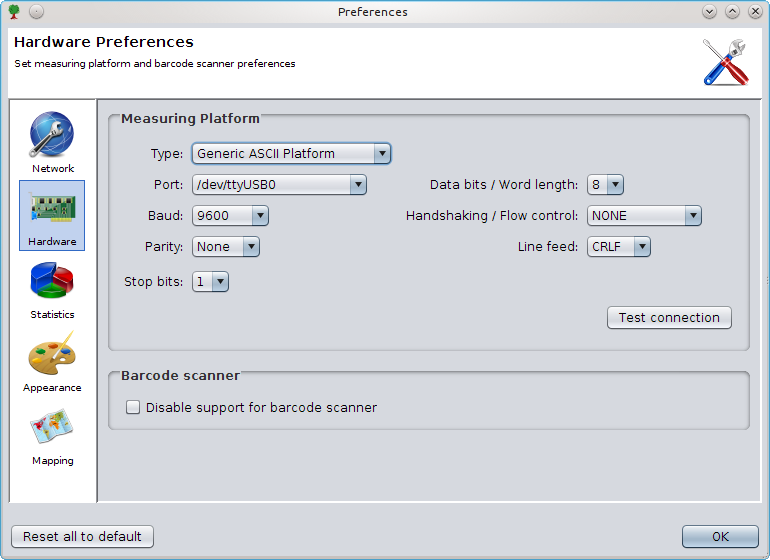
\includegraphics[width=0.6\textwidth]{Images/hardwareprefs.png}
    \caption{The hardware preferences dialog.}
    \label{fig:hardwareprefs}
\end{figure}

In the type pull down menu, select the type of measuring equipment you are using. Note that this refers to the equipment that the computer is attached to, and not necessarily the measuring platform itself. For instance, Velmex platforms are typically connected through a Metronics digital readout device. Included in this list is the EveIO device which is an open-source device designed for the Cornell Tree-Ring Laboratory. Circuit drawings for this device can be obtained from the Cornell lab to enable Hensen measuring platforms to be used with Tellervo (and other software).  If you measuring platform is not included in the list it should be relatively easy for us to add support so please get in touch and we'll see what we can do.  Alternatively you could implement support yourself (either personally or by employing an independent developer).  Technical details on how to do this are included in section \ref{txtSupportingNewMeasuringPlatforms}, page \pageref{txtSupportingNewMeasuringPlatforms}.  

Next you must choose the port that your platform is connected to from the pull down menu. In Windows this will be a COM port, in Linux and Mac this will be a /dev/xxx port.  Depending on the type of platform you choose, you may also need to set various communication parameters.  If these boxes are enabled, please check the documentation that came with your measuring platform to ensure these values are set correctly.

To check whether your platform is working, click the `Test connection' button (see figure \ref{fig:hardwaretest}) and attempt to measure a few rings.  Different measuring platforms have different capabilities.  For instance, some include a physical switch for firing measurement events, others also include switches for resetting measurements to zero.  Some platforms (e.g. Lintab) also continuously report the measurement values to the computer.  So depending on the hardware you use, Tellervo will present the you with slightly different options.  

\begin{wrapfigure}{r}{0.5\textwidth}
  \begin{center}
    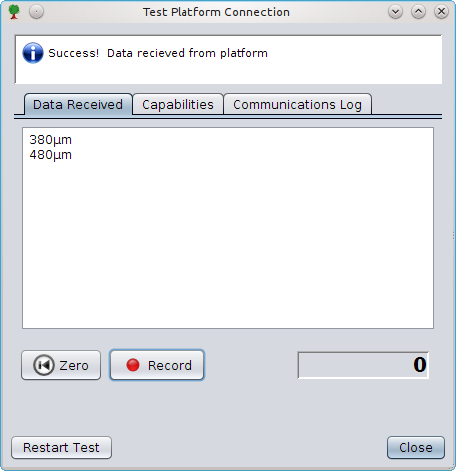
\includegraphics[width=0.48\textwidth]{Images/hardwaretestdialog.png}
  \end{center}
    \caption{Testing the connection to a hardware measuring platform.}
    \label{fig:hardwaretest}
\end{wrapfigure}



The test dialog includes information about the capabilities of your platform as well as a log window to show the raw information being received by Tellervo.  If you are having trouble interfacing with your platform, you should send the communications log to the developers, along with as much information about your hardware as possible.

Once you are satisfied that you are getting the correct results from the measuring platform, click close on the test window and then close the preferences dialog to return to the Tellervo home screen.





